\chapter{Funzioni}

Tra le relazioni binarie, cioè su una coppia di insiemi, alcune hanno una particolare importanza: le funzioni. 
Le funzioni sono relazioni tra gli elementi di un insieme $D$ e di un insieme $C$ tali che ad ogni elemento dell’insieme $D$ corrisponda esattamente un elemento di $C$.
In altre parole, una corrispondenza tra gli elementi di $D$ e quelli di $C$ è una funzione quando:
\begin{enumerate}
    \item Ogni elemento di $D$ ha un corrispondente in $C$;
    \item Nessun elemento di $D$ ha più di un corrispondente in $C$.
\end{enumerate} 
\begin{definition}[Funzione]
    Una relazione $R\subseteq DxC$ si dice funzione se per ogni $a\in D$ esiste uno ed un solo $b\in C$ tale che $(a, b)\in R$.
\end{definition}

Il primo insieme, $D$, si dice \textbf{dominio} di $f$, il secondo, $C$, \textbf{codominio}. A ciascun elemento $x$ del dominio della $f$ corrisponde un’(unica) \textbf{immagine}, indicata da $f(x)\in C$. Analogamente, si dice che $x\in D$ è \textbf{controimmagine} di $f(x)\in C$.

\begin{definition}[Funzione immagine]
    Data la funzione $f:D\rightarrow C$, l’insieme $Im(D)\subseteq C$ costituito dalle immagini degli elementi di $D$ si dice insieme delle immagini di $f$.
\end{definition}

\begin{example}\label{es:funzioni1}
    Consideriamo le relazioni rappresentate da:
    \begin{figure}[ht]
        \centering
        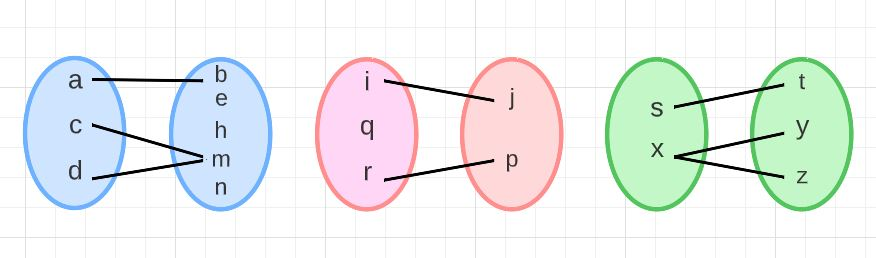
\includegraphics[width = 9cm]{images/funzioni_es.JPG}
        \caption{Quali tra queste è una funzione?}
        \label{fig:es:func}
    \end{figure}
    
    Stando a quanto detto solo la prima è una funzione, perchè le altre due non rispettano la sua definizione.
\end{example}

\section{Classificazione delle funzioni}
Nel paragrafo precedente abbiamo notato (grazie all'Esempio \ref{es:funzioni1}) che la condizione di funzione non implica che due distinti elementi del dominio abbiano immagini distinte o che gli elementi del secondo insieme abbiano una controimmagine nel dominio.

Quelle funzioni che rispettano una di queste, o altre, condizioni vengono indicate con denominazioni specifiche.
\begin{definition}[Iniettiva]
    La funzione $f: D\rightarrow C$ si dice iniettiva se per ogni $x_1\in D$ e $x_2\in D$, con $x_1\neq x_2$, si ha che $f(x_1)\neq f (x_2)$.
    
    Dunque una funzione $f: D\rightarrow C$ si dice iniettiva se nessun elemento di $C$ è dotato di più di una controimmagine in $D$.
\end{definition}

\begin{definition}[Surriettiva]
    La funzione $f: D\rightarrow C$ si dice suriettiva se per ogni $b\in C$ esiste (almeno) un $x\in D$ tale che $f(x) = b$.
    
    Dunque una funzione $f: D\rightarrow C$ si dice suriettiva se ogni elemento dell’insieme $C$ ha (almeno) una controimmagine nel dominio.
\end{definition}

\begin{definition}[Biiettiva]
    La funzione $f: D\rightarrow C$ si dice biiettiva se è contemporaneamente iniettiva e suriettiva.
\end{definition}

\begin{example}
    La funzione $R1: A\rightarrow B$ introdotta nell’Esempio \ref{es:funzioni1} non è iniettiva, in quanto ai due (distinti) elementi del dominio, corrisponde la stessa immagine. 
    Essa non è suriettiva, in quanto gli elementi del secondo insieme, $h$ ed $n$, non hanno alcuna controimmagine nel dominio $A$. 
    Non essendo iniettiva (nè suriettiva), la funzione non è certamente biiettiva.
\end{example}

\section{Numerabilità}
\begin{definition}[Numerabilità]
    Si dice numerabile qualunque insieme che ha una corrispondenza biunivoca con i numeri naturali.
\end{definition}

\begin{exercise}[$\mathbb{N}x\mathbb{N}$ è numerabile]
    
    Dati due insiemi $\mathbb{N}$ ed $\mathbb{N}x\mathbb{N}$ dimostriamo che la funzione $\mathbb{N}x\mathbb{N}$ è numerabile.
    L'unico modo per dimostrarlo è rappresentarlo tramite una tabella a coda di colombo. 
    
    \setlength{\tabcolsep}{13pt}
    \renewcommand{\arraystretch}{1}
    \begin{table}[ht]
        \centering
        \begin{tabular}{|c||c|c|c|c|c|c}
             \hline \textbf{N}&\textbf{0}&\textbf{1}&\textbf{2}&\textbf{3}&\textbf{4}&\textbf{5}\\\hline\hline
            \textbf{0}    &0&2&5&9&14&20\\\hline
            \textbf{1}    &1&4&8&13&19&26\\\hline
            \textbf{2}    &3&7&12&18&25&33\\\hline
            \textbf{3}    &6&11&17&24&32&...\\\hline
            \textbf{4}    &10&16&23&31&...&\\\hline
            \textbf{5}    &15&22&30&...&&
        \end{tabular}
        \caption{Dimostrazione con coda di colombo}
        \label{tab:numerab}
    \end{table}
    
    Come notiamo in tabella \ref{tab:numerab}, numerando le caselle lungo le diagonali opposte, gli intervalli saranno sempre finiti. In tutti gli altri casi ciò non accade perchè si presentano sempre intervalli infiniti che bloccano la nostra iterazione.
    
\end{exercise}

\begin{exercise}[$P(\mathbb{N})$ non è numerabile]
    
    Prima di dimostrarlo, aggiungiamo due definizioni:

    \begin{definition}[Funzione booleana]
        
        La funzione booleana è un insieme formato da coppie di valori: elemento e valore booleano.
        $f=\{\mathbb{N}\rightarrow bool\}$
    \end{definition}

    \begin{definition}[Funzione caratteristica]
        
        La funzione caratteristica è una funzione che ritorna 1 se l'elemento che si considera appartiene all'insieme, altrimenti ritorna 0. 
        \end{definition}

        Dimostriamo ora quanto scritto nell'assunto di partenza. Procediamo per assurdo supponendo che $P(\mathbb{N})$ sia numerabile.

        Dato che esiste una corrispondenza biunivoca tra $\mathbb{N}$ e $P(\mathbb{N})$ posso rappresentare in una tabella formata da sequenze di 0 e 1 un esempio del problema.
    
        \setlength{\tabcolsep}{13pt}
        \renewcommand{\arraystretch}{1}
        \begin{table}[ht]
            \centering
            \begin{tabular}{|c||c|c|c|c|c|c|c}
                 \hline \textbf{N}&\textbf{0}&\textbf{1}&\textbf{2}&\textbf{3}&\textbf{4}&\textbf{5}&\textbf{6}\\\hline\hline
                 \textbf{0}&\textbf{0}&1&0&1&...&&\\\hline
                 \textbf{1}&1&\textbf{1}&0&1&0&...&\\\hline
                 \textbf{2}&0&0&\textbf{0}&1&1&1&...\\\hline
                 \textbf{3}&1&1&0&\textbf{0}&0&0&1\\\hline
                 \textbf{4}&...&0&1&1&\textbf{0}&1&1\\\hline
                 \textbf{5}&&...&0&0&1&\textbf{0}&0\\\hline
                 \textbf{6}&&&...&1&1&0&\textbf{0}
            \end{tabular}
            \caption{Dimostrazione per diagonalizzazione}
            \label{tab:non_numerab}
        \end{table}
        
        Seguendo la tabella \ref{tab:non_numerab}, identifichiamo con $D$ l'insieme formato dagli elementi della diagonale e con $\overline{D}$ il suo complementare (ogni elemento di $\overline{D}$ è l'opposto rispetto a $D$).

        Notiamo ora come, essendo la tabella infinita, prima o poi l'insieme $\overline{D}$ sarà uguale ad una colonna.
        Quindi in qualche punto della tabella $D$ e $\overline{D}$ avranno lo stesso valore.

        Ecco trovaro l'assurdo perché due insiemi complementari non possono avere alla stessa posizione un valore uguale.

        Abbiamo quindi dimostrato per \textbf{diagonalizzazione} che l'insieme $P(\mathbb{N})$ non è numerabile perché non è biunivoco.
    \end{exercise}